\documentclass[11pt,a4paper]{article}
\usepackage[margin=1in]{geometry}
\usepackage{graphicx}
\usepackage{booktabs}
\usepackage{hyperref}
\usepackage{enumitem}
\usepackage{amsmath}
\usepackage{amssymb}
\usepackage{float}
\usepackage{xcolor}
\graphicspath{{../figures/}}

\title{MLOps Report: IMDb Sentiment Analysis}
\author{UPC MLOps Team}
\date{\today}

\begin{document}

\begin{titlepage}
  \centering
  \vspace*{3cm}
  {\Huge \textbf{MLOps Report}}\\[0.8cm]
  {\LARGE IMDb Sentiment Analysis}\\[1.5cm]
  {\Large UPC MLOps Team}\\[0.5cm]
  {\large \today}\\[4cm]
  
\includegraphics[width=0.4\textwidth]{fib-upc-logo.png}\\[1cm]
  {\large Machine Learning Operations -- Academic Year 2024/2025}
\end{titlepage}

\tableofcontents
\newpage

\section{Introduction}
\subsection{Goal of the Project}
The project delivers an end-to-end analytics platform that ingests comment sections from major movie-review websites, filters noise such as spam or off-topic content, and extracts sentiment signals that can support downstream dashboards. Starting from the \texttt{cookiecutter-data-science} template, we built a reproducible pipeline that downloads the IMDb benchmark dataset, cleans and vectorises text, trains a logistic regression model, and evaluates it against held-out examples. The success criteria agreed during inception were:\begin{itemize}[leftmargin=*]
  \item Produce sentiment metrics (accuracy, F1) above 0.85 while maintaining resilience to noisy inputs (spam-filtering and HTML stripping).
  \item Reproduce the full data and model workflow via DVC with a single \texttt{dvc repro}.
  \item Track experiments (hyperparameters, metrics, artefacts, emissions) in MLflow to support iterative analysis of comment streams.
\end{itemize}
The latest evaluation run (see Section~\ref{subsec:milestone2}) satisfies these targets, with the logistic regression classifier reaching 0.894 accuracy and 0.895 F1.

\section{Methodology}
\subsection{Milestone 1: Inception}
\subsubsection{Problem Selection and Requirements}
We selected binary sentiment classification for IMDb reviews because it combines natural language processing with clear business value (gauging audience sentiment) and publicly available benchmark data. Functional requirements include batch scoring of text reviews and traceable metrics. Non-functional requirements emphasise reproducibility, energy-awareness, and compatibility with container deployment.

\subsubsection{Dataset Card Summary}
The dataset card (\texttt{data/README.md}) follows the Hugging Face template. It documents:\begin{itemize}[leftmargin=*]
  \item \textbf{Provenance and Licence:} IMDb reviews under the IMDb Terms of Use, crowdsourced annotations, English-only content.
  \item \textbf{Composition:} 50,000 labelled reviews (25k train / 25k test), binary sentiment.
  \item \textbf{Motivation and Uses:} Benchmarking sentiment analysis models, educational demonstrations, not suitable for nuanced or multilingual sentiment.
  \item \textbf{Collection Process:} Neutral reviews excluded, balance enforced between polarities.
  \item \textbf{Limitations \& Biases:} Domain specificity, possible demographic bias, binary simplification of sentiment.
  \item \textbf{Citation:} Maas et al. (2011) reference for reproducible acknowledgement.
\end{itemize}

\subsubsection{Model Card Summary}
The model card (\texttt{models/README.md}) captures:\begin{itemize}[leftmargin=*]
  \item \textbf{Model Description:} TF--IDF features with a scikit-learn logistic regression classifier.
  \item \textbf{Intended Uses:} Baseline benchmarking and teaching reproducible MLOps practices; not for high-stakes production.
  \item \textbf{Training Procedure:} 25k train / 25k test split, TF--IDF with 1--2 grams, logistic regression (liblinear solver).
  \item \textbf{Evaluation:} Accuracy and F1 typically above 0.82, with current run at 0.894/0.895.
  \item \textbf{Limitations and Ethics:} English-only, binary polarity, sensitivity to sarcasm, potential demographic bias.
\end{itemize}

\subsubsection{Project Coordination and Communication}
We operate with a lightweight Scrum cadence: weekly planning and review ceremonies guide backlog priorities, while daily asynchronous stand-ups surface blockers. Slack hosts coordination, and its GitHub and Jira integrations post activity notifications and ticket updates into a shared channel, keeping sprint status visible despite distributed schedules.

\subsubsection{Selection of Cloud Provider}
For Milestone~4 we plan to deploy the inference service on Google Cloud Run. Its fully managed container runtime, integration with Artifact Registry, and generous free tier make it a pragmatic choice for lightweight academic workloads while providing a path to autoscaling if needed.

\subsection{Milestone 2: Model Building -- Reproducibility}\label{subsec:milestone2}
\subsubsection{Project Structure}
The repository inherits the \texttt{cookiecutter-data-science} scaffold, separating code under \texttt{mlops\_imdb/}, configuration in \texttt{params.yaml}, data artefacts under \texttt{data/}, and generated reports beneath \texttt{reports/}. This consistent layout eases onboarding and tooling integration.

\subsubsection{Code Versioning}
We apply GitHub Flow on top of the enforced branch naming convention (\texttt{feature/}, \texttt{fix/}, \texttt{chore/}, \texttt{docs/}, \texttt{experiment/}). Conventional Commit messages feed changelogs and are validated via PR automation (Section~\ref{sec:collab}).

\subsubsection{Data Versioning}
DVC stages (\texttt{prepare} $\rightarrow$ \texttt{features} $\rightarrow$ \texttt{train} $\rightarrow$ \texttt{eval}) encode dependencies and outputs. Regenerating the pipeline uses \texttt{dvc repro}, guaranteeing deterministic artefact creation (\texttt{data/processed}, \texttt{models/}, \texttt{reports/metrics.json}, figures).
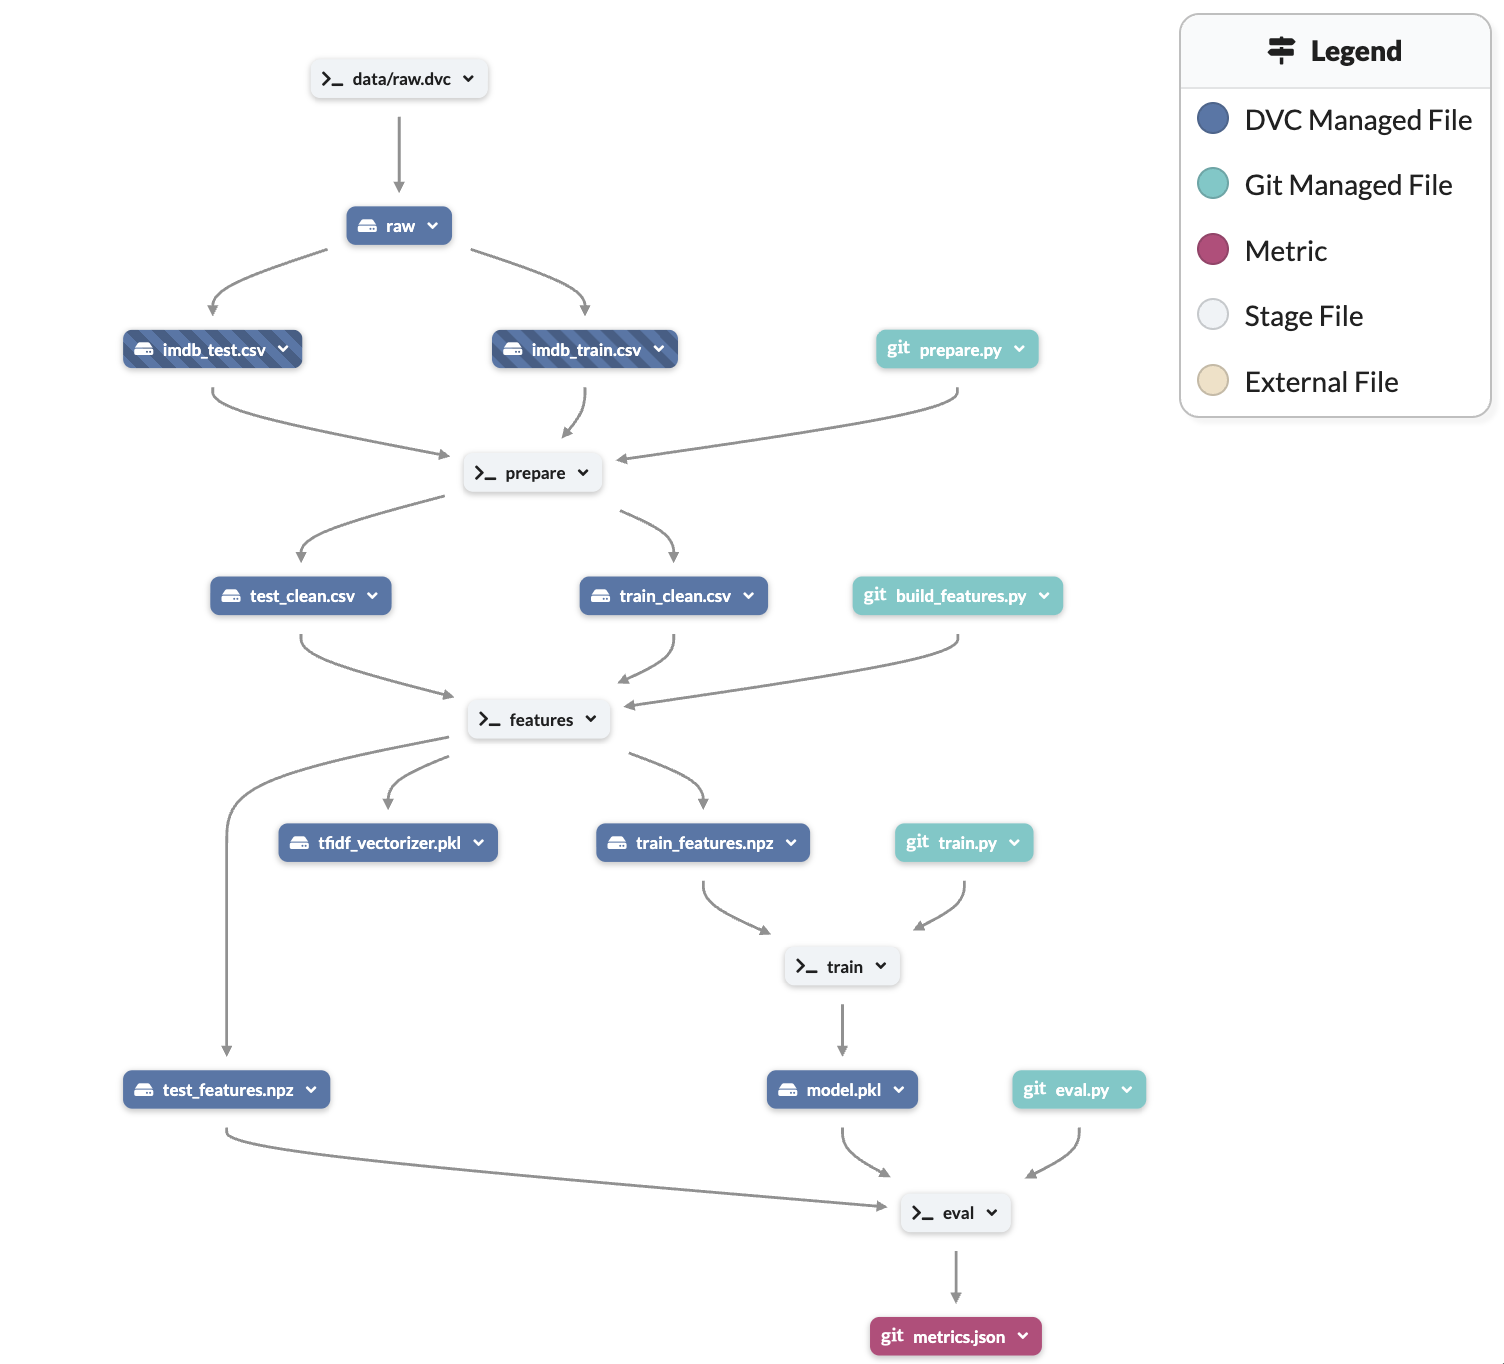
\includegraphics[width=1\textwidth]{dvc_pipeline.png}
\subsubsection{Experiment Tracking}
MLflow is configured through \texttt{mlops\_imdb/config.py}. Both training and evaluation stages wrap their execution in \texttt{mlflow.start\_run}, logging hyperparameters, dataset dimensions, metrics, confusion-matrix artefacts, and CodeCarbon emissions under the shared \texttt{emissions\_kg} metric. Local runs default to \texttt{./mlruns}, while remote tracking URIs can be supplied via environment variables.

\subsubsection*{Evaluation Results}
Table~\ref{tab:metrics} summarises the most recent evaluation metrics sourced from \texttt{reports/metrics.json}. The confusion matrix in Figure~\ref{fig:cm} reveals a balanced error profile across classes.

\begin{table}[H]
  \centering
  \caption{IMDb test performance (logistic regression baseline).}
  \label{tab:metrics}
  \begin{tabular}{lcccc}
    \toprule
    Metric & Accuracy & Precision & Recall & F1-score \\
    \midrule
    Value & 0.8943 & 0.8907 & 0.8990 & 0.8948 \\
    \bottomrule
  \end{tabular}
\end{table}

\begin{figure}[H]
  \centering
  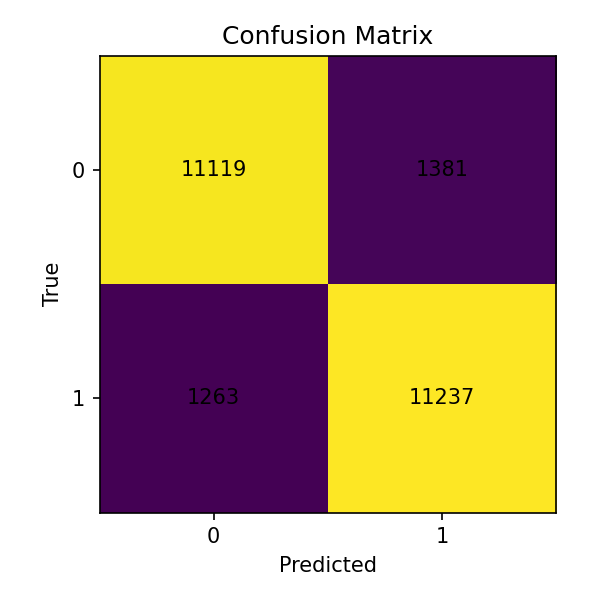
\includegraphics[width=0.75\textwidth]{baseline_confusion_matrix.png}
  \caption{Confusion matrix on the IMDb test split.}
  \label{fig:cm}
\end{figure}

\subsection{Milestone 3: Model Building -- Quality Assurance}
\subsubsection{Energy Efficiency Awareness}
CodeCarbon contexts wrap every DVC stage. The run captured in \texttt{reports/codecarbon\_emissions.csv} emitted 7.15\,mg CO\(_2\)eq over 27.1\,seconds (Table~\ref{tab:carbon}), with feature generation dominating the footprint. Emission figures are logged back to MLflow, enabling longitudinal monitoring.

\begin{table}[H]
  \centering
  \caption{CodeCarbon emissions per stage (mg CO\(_2\)eq).}
  \label{tab:carbon}
  \begin{tabular}{lcc}
    \toprule
    Stage & Duration (s) & Emissions (mg) \\
    \midrule
    Prepare data & 5.51 & 1.21 \\
    Build features & 14.46 & 5.52 \\
    Train model & 3.47 & 0.21 \\
    Evaluate model & 3.63 & 0.22 \\
    \midrule
    \textbf{Total} & 27.07 & \textbf{7.15} \\
    \bottomrule
  \end{tabular}
\end{table}

\subsubsection{Static Code Analysis}
Ruff enforces formatting and linting (line length 99, import sorting, code-style checks). The CI pipeline (CI/CD Automation in Milestone 5) runs \texttt{uv run ruff format --check} and \texttt{uv run ruff check} on every push and pull request.

\subsubsection{Model Testing}
Pytest suites validate the training and evaluation flows using synthetic sparse matrices (see \texttt{tests/modeling/}). Assertions confirm persisted models expose coefficients, metrics JSON contains expected fields, and confusion matrices are rendered as PNG files.

\subsubsection{Data Testing}
Data preparation tests (\texttt{tests/data/test\_prepare.py}) exercise schema validation and text-cleaning behaviours, while \texttt{tests/data/test\_download\_imdb.py} mocks the dataset download to assure reproducible CSV outputs. Although we do not yet employ Great Expectations, these lightweight checks catch regressions in preprocessing logic.

\end{document}
